\section{Filter Parameters}
Given the project specifications, it is possible to draw the \textbf{Data Flow Diagram} as shown in \autoref{lab1:fig:iir-dfd}.
\begin{figure}[htbp]
	\center
	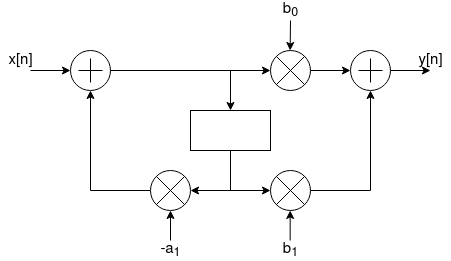
\includegraphics[width=0.65\textwidth]{chapter1/images/iir-dfd.png}
	\caption{Target filter data flow diagram}
	\label{lab1:fig:iir-dfd}
\end{figure}

Given the basic structure, it is necessary to determine the values of the $a$ and $b$ parameters. After feeding the specifications in the provided Matlab script \texttt{myiir\_design.m}, the results are:
\begin{align}
    a &= [-21] \\
    b &= [53,\ 53]
\end{align}


As defined in the project specifications, the filter is going to be implemented in hardware and will use an 8 bit \textbf{fixed point} representation: this simplifies the structure of the filter, but limits its precision.\\
To properly verify the functionality of the filter, it is necessary to have a reference model that also works with 8 bit fixed point numbers. In addition, this allows for an insightful comparison of the filter's behavior when it is working in floating point (in Matlab) versus fixed point.
%, which is going to be implemented in C. (detto subito dopo)
Truly fixed point operation is modeled in a C program where coefficients and data are stored using the standard \texttt{int} data type. A scale factor equal to $2^{n_b-1}$ is implied and input values to this program are rescaled within the same Matlab script where they are generated in order to match the full scale range of an $n_b$-bits two's complement representation.  The loss in precision arising from truncating the $n_b-1$ least significant bits at the output of every hardware multiplier is simulated in C using the right-shift operator \texttt{>>}.

Rounding the input samples to the closest representable value according to the adopted bitwidth is a nonlinear operation that introduces distortion in the signal, producing spurious harmonics on top of the pure sinusoidal wave expected at the output of a linear filter. The relevant parameter to characterize this effect is the \textit{total harmonic distortion} (THD). The dependence of the THD on the internal bitwidth has been calculated from simulations, with the results reported in figure \ref{fig:thdplot}. 

%If the internal representation is the same as the one prescribed for the interface ($n_b=8$), then the THD output spectrum is as shown in figure \ref{fig:thd8bit}.
% TODO: correggere questa immagine
%\be<gin{figure}
%	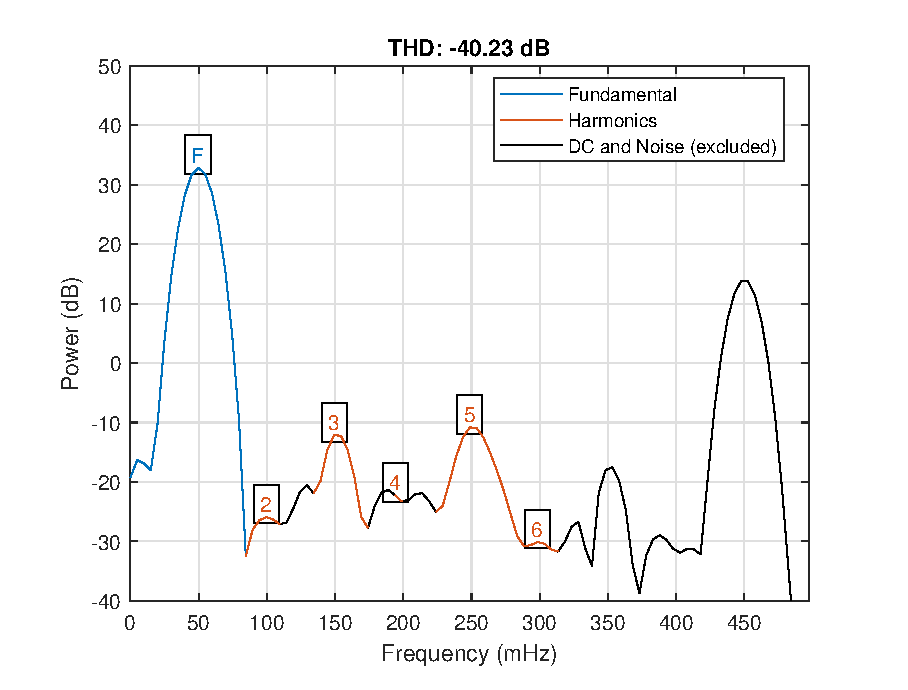
\includegraphics[width=\textwidth]{./chapter1/images/thd_with_8b.eps}
%	\caption{Spectrum and total harmonic distortion ($n_b=8$)}
%	\label{fig:thd8bit}
%\end{figure} 

From these results we conclude that the smallest implementation in terms of area occupied by arithmetic operators requires $n_b=7$ in order to keep the total distortion below $-30\,\textrm{dBc}$, as requested by the specifications.

\section{Hardware design}
The computational structure adopted for this project is the direct form II, whose DFG is in figure \ref{fig:arch_schematic}. This graph is the mapping of the following discrete-time equations:
\begin{align}\label{eqn:iir2}
&w(n) = x(n) - a_1w(n-1)\\
&y(n) = b_0v(n) + b_1v(n-1)
\end{align} 
\subsection{Internal parallelism}
\subsubsection{Accuracy}
From a preliminary investigation regarding the dependence of THD on the representation accuracy, which is linked to $n_b$, we found that $n_b=7$ is enough to meet the requirements. This means that dropping the least significant bit from the input samples (represented on 8 bits) can simplify internal computations with an acceptable degradation in performance. The previous analysis has been carried out using a model where numbers include $n_b-1$ fractional bits (the binary digits with weights $2^{-1}$, $2^{-2}$, ..., $2^{n_b-2}$), therefore we can expect that allocating 6 fractional bits for all the internal variables in the VHDL implementation will provide enough accuracy for our purposes.
\subsubsection{Avoiding overflow}
 The C reference model is accurate in predicting the error introduced by truncation, which affects the output of every multiplier block, but it neglects the inability to represent a number larger than 1 with the only integer bit available in the standard fixed-point format. An overflow condition may occur in intermediate steps of the computation where the result would require more than one integer bit. In order to determine the right sizing that guarantees the absence of overflow, the maximum value of the intermediate variable $w(n)$ must be determined. Using eq. \ref{eqn:iir2},
\begin{equation*}
w(n) = \sum_{i=0}^{n} (-a_1)^i x(n-i)
\end{equation*}
Hence, assuming $|x(n)|\leq 1$,
\begin{equation*}
|w(n)|\leq \sum_{i=0}^{n} |(-a_1)^i x(n-i)| \leq \sum_{i=0}^{n} |a_1|^i \leq \frac{1}{1-|a_1|} \approx 1.2 
\end{equation*}
According to this computation, two integer bits are enough to avoid overflow at the nodes where $w(n)$ is processed within the DFG. Consequently, the adder and multiplier in the feedback loop on the left side in figure \ref{lab1:fig:iir-dfd} will operate on inputs with 2 integer bits and 6 fractional bits, as already determined by the previous reasoning on the internal accuracy. 
As for the operators in the feedforward part (on the right side of the DFG), multiplying $w(n)$ and $w(n-1)$ by $b_1$ and $b_2$ will always produce a result lower than 1 in magnitude, for which a single digit to the left of the radix point suffices. Therefore the output of those multiplier is resized to match the same format used by the final adder consisting of 1 integer and 6 fractional bits. The eighth digit, which is always zero, is appended to the final result, thus becoming its LSB, to comply with the specified interface format. A summary of the internal parallelism used throughout the filter is reported in figure \ref{lab1:fig:parallelism}.
\begin{figure}
	\makebox[\textwidth][c]{
	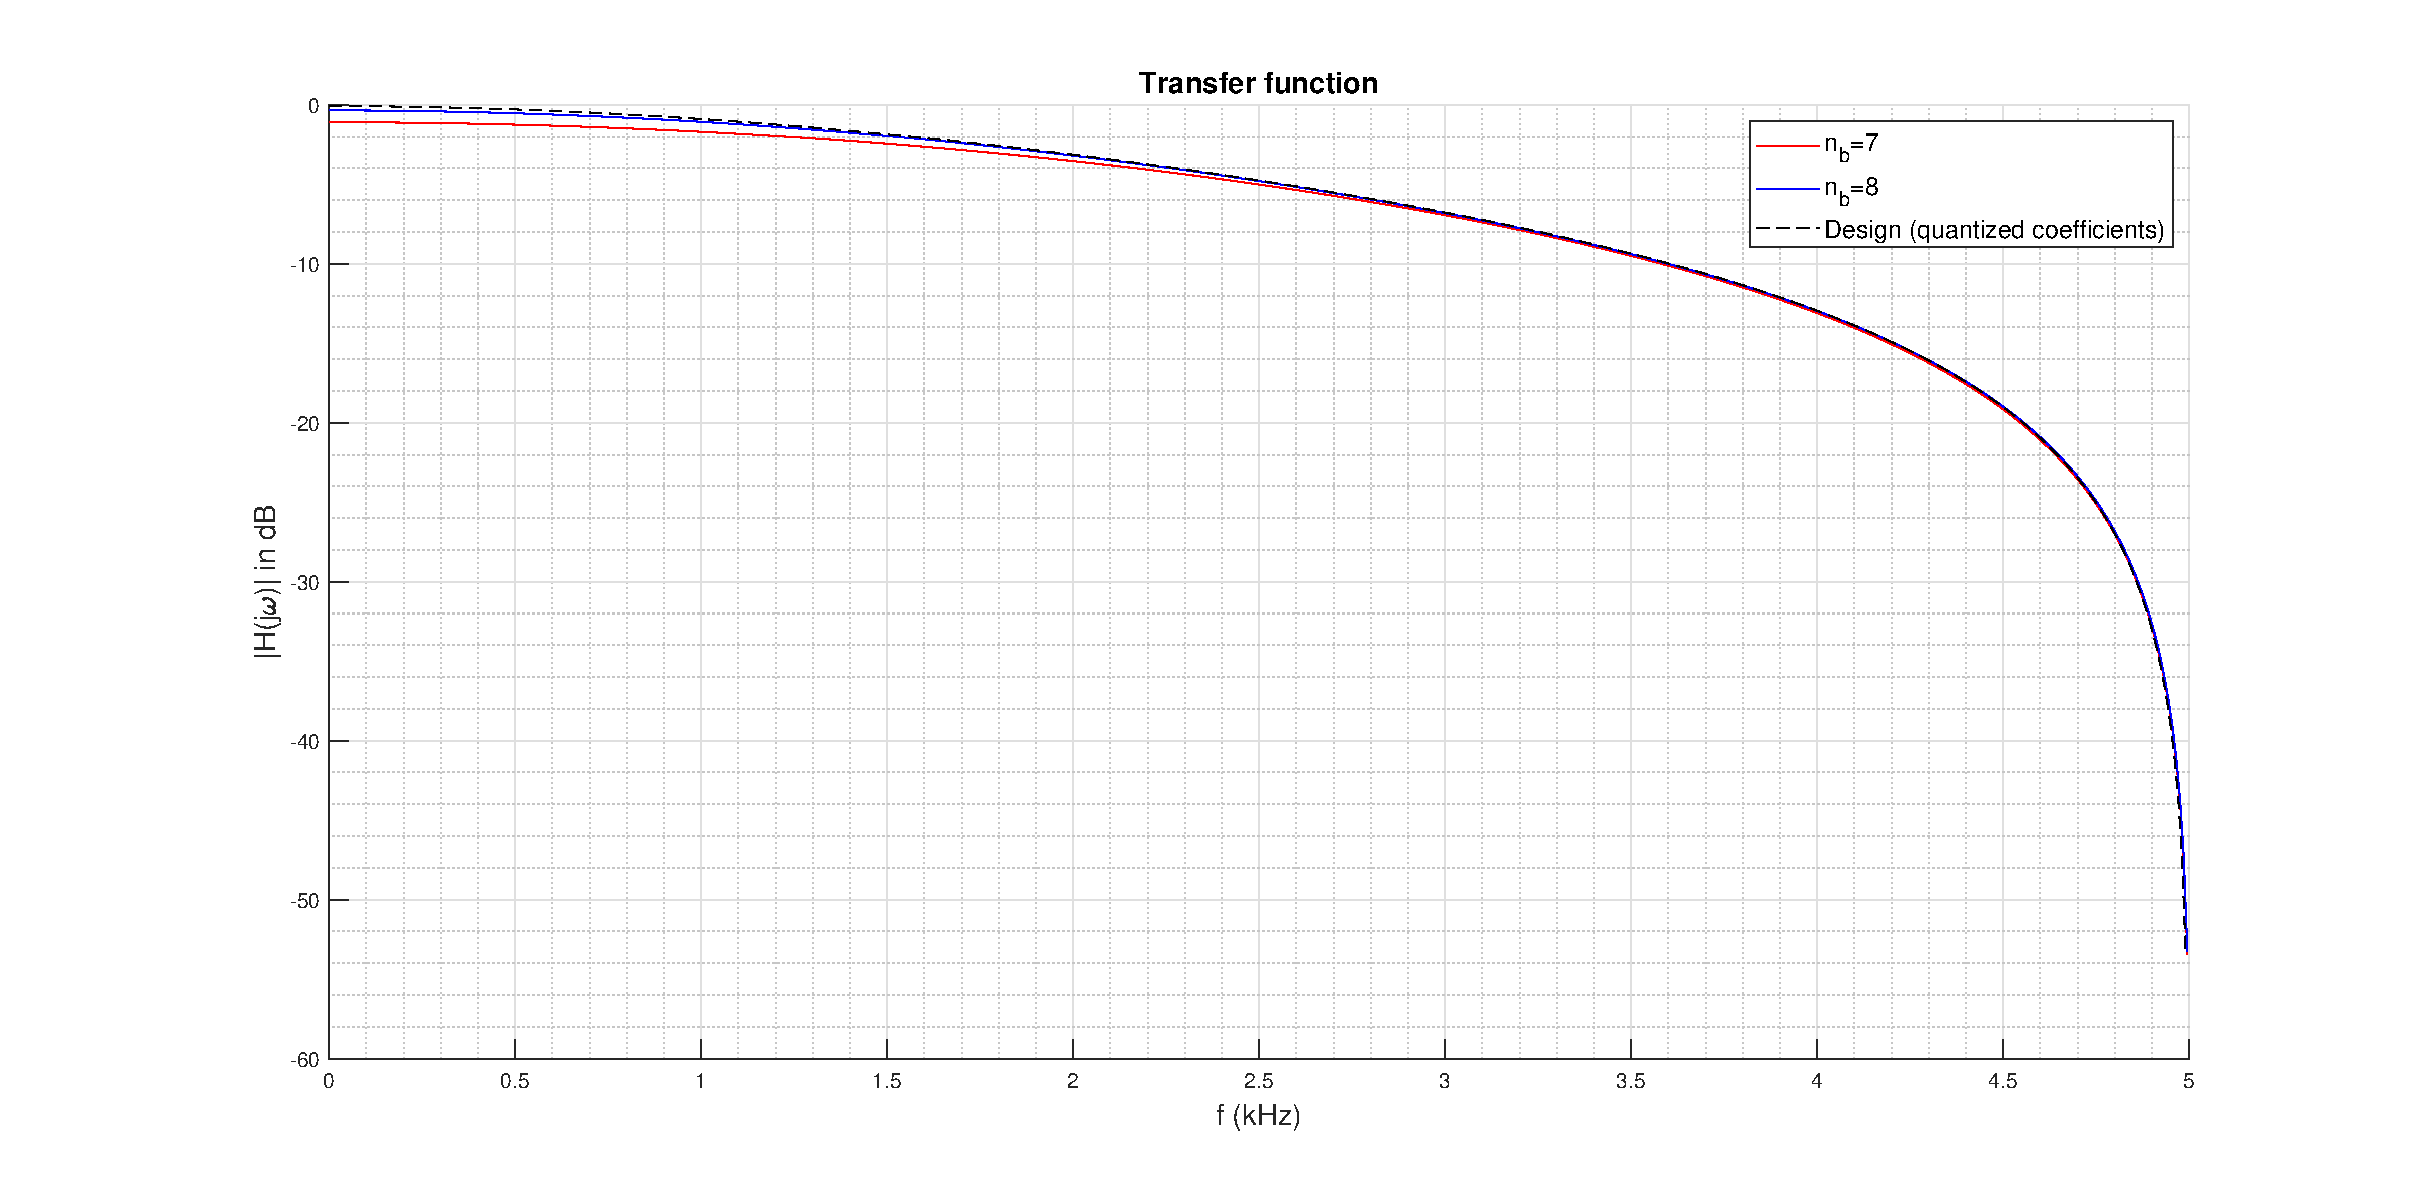
\includegraphics[width=1.5\textwidth]{./chapter1/images/tf_comparison.eps}}
	\caption{Transfer function for a few values of $n_b$}
	\label{fig:tfcomparison}
\end{figure}
\begin{figure}
	\makebox[\textwidth][c]{
	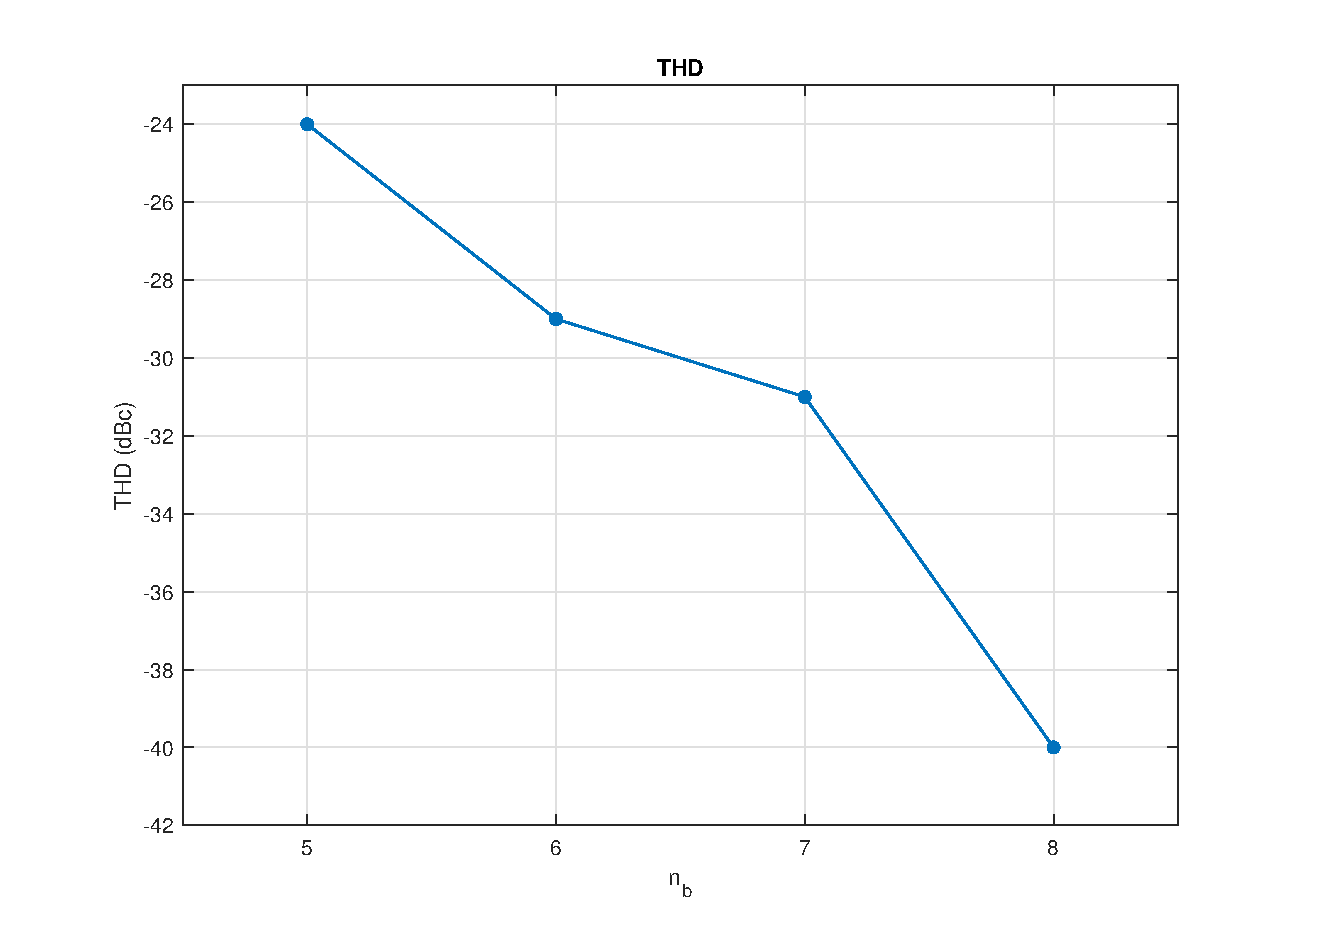
\includegraphics[width=1.2\textwidth]{./chapter1/images/thdplot.eps}}
	\caption{THD as a function of $n_b$}
	\label{fig:thdplot}
\end{figure}

\section{Verification}
\subsection{Methodology}
The task of verifying a design using a logical simulator such as ModelSim can be broken down into three distinct phases: first of all the generation of suitable input vectors, then a number of logical simulator runs where the device-under-test is operated within a testbench environment that drives its inputs while monitoring its outputs, and finally the analysis of output data both in terms of agreement with a reference behavioral implementation and performance as measured according to the FOMs that are relevant to the specific application.

\paragraph{Targets} In order to plan the verification flow, all aspects of the design that need to be tested must be identified. In the case of a data processing unit like the one we are considering, the correctness of the \textbf{output data} stream must be checked along with the \textbf{timing} of every control and status signal.

\paragraph{VHDL testbench structure} The testbench is made up of the following non-synthesizable components:
\begin{itemize}
	\item Clock generator (\texttt{clkGen.vhd}): it generates a clock signal whose period is parametrized by a constant written externally in a dedicated package (\texttt{work.simconsts}).
	\item Data generator (\texttt{dataGen.vhd}): it fetches the input samples from a text file to feed the DUT at regular intervals, with a frequency submultiple of $f_{clk}$.
	\item Monitor (\texttt{dataSink.vhd}): it collects output samples in a text file for further analysis and verifies that the status signal \texttt{VOUT} is asserted with the right timing. This is done by probing the control signal \texttt{VIN} and ensuring that \texttt{VOUT} is issued after a latency period (in clock cycles) given as a constant and dependent on the internal architecture. If any unexpecyed behavior is detected, a warning message appears on the output log.
\end{itemize}

\paragraph{Data generation and analysis} For the creation of the input samples file we resorted to an automated script that provides several options to generate waveforms such as the impulse, the unit step, a sinewave or a chirp signal whose parameters (frequency and amplitude) are given as arguments. Once the input data is stored in a text file, suitable commands are issued to run a simulation in ModelSim. Finally, the output of the monitor component is checked against the stream produced by the reference C model. 

\subsection{Results}